\chapter{Selection Application}
\label{sec:selection_application}

This chapter describes the of the selection application used for this work. After a rundown of third party requirements and a summary of relevant C++ classes, the description is further subdivided according to its abstract, key requirements.
The goal of this chapter is to describe how the application, especially the Octree\cite{Octree}, is designed and implemented. Accordingly, key lines of source code as well as plenty of explanatory comments are provided.

\section{Additional third party libraries}
\label{sec:additional_third_party_libraries}

% @TODO climberpi mesh saliency einbauen incl Verlinkung im libfile

To ensure a scalable, platform independent implementation of the application, the following third party libraries, frameworks and APIs are used.

\subsection{OpenGL}
\label{sec:opengl}

The Open Graphics Library OpenGL \cite{OpenGL} is a powerful industry standard API for rendering 2D and 3D graphics, independently of programming language and operating system. One of its most outstanding features is its ability to directly perform operations on the graphics processing unit of a computer, allowing fast, hardware-accelerated display of graphic elements. For this work, OpenGL is used for displaying the 3D objects both in the user study and throughout development of the selection application. The task of displaying rendered images across multiple projection surfaces on a 360\degree panorama view is handled by software developed at the Zentrum f\"ur Virtuelle Realit\"at und Visualisierung (V2C) of the Leibniz-Rechenzentrum \cite{v2c}.

OpenGL is based on the following basic structures and concepts:

\begin{description}
	\item[Vertex Buffer Objects] (VBOs) contain actual vertex data. Coordinates, normal and color information, texture mapping and any other kind of data that is desired can be saved in these kinds of objects. They are designed as buffer objects to be stored directly within the memory of the video card, ensuring extremely fast access times.
	\item[Vertex Array Objects] (VAOs) are objects which can contain one or more Vertex Buffer Objects and store information for complete, rendered objects. In other words, VAOs store descriptions of vertex data stored in VBOs. For example, the number of coordinates the vertices are made of, in which order etc. From a performance aware point of view, they are a great improvement over older, deprectecated concepts in OpenGL since multiple calls to bind and upload distinct sets of data belonging to the same object to the graphics processing unit can be bundled in one call to a VAO.

	\item[Vertex Shaders] are small pieces of C-like code, executed by the graphics card, which can perform extremely fast, basic operations on every vertex of a vertex data input stream. Vertex shaders are one of two mandatory types of shaders. As soon as an openGL \texttt{draw} command is called, they process every incoming vertex and output two things for each one: Its position (untouched or altered in any way desired) within the output window on screen, and a set of arbitrary defined custom data such as normal information, color and texture mapping. These attributes are calculated on a per-vertex basis.

	\item[Fragment Shaders] complete the absolute minimum for an openGL-based rendering pipeline to be able to display anything, together with vertex shaders. They are executed per pixel and, therefore, considerably more often than vertex shaders. Their purpose is to interpolate, for each pixel in between vertices, its RGB value, based on the per-pixel values calculated by the vertex shader. The term \textit{fragment} is often informally described as a \textit{potential pixel}, as the final RGB value of a pixel can still be changed after it is processed by the fragment shader.

\end{description}

\subsection{GLUT}
\label{sec:glut}

As stated on its official webpage \cite{GLUT}, GLUT is an official OpenGL Utility Toolkit which provides, among other features, support for multiple windows, control of such windows and handling input from devices such as keyboards and mouses. It is commonly used to achieve interactive windows with cross-platform compatibility displaying rendered images produced by OpenGL. Handling input via the handheld controller in the user study is achieved with the help of GLUT during this work.

\subsection{GLEW}
\label{sec:glew}

The OpenGL Extension Wrangler Library (GLEW)\cite{GLEW} is a cross-platform extension loading library, specifically designed to be used by C/C++ applications. It provides run-time mechanisms for OpenGL extensions supported on the target platform, allowing to faster query and load those extensions.

\subsection{ASSIMP}
\label{sec:assimp}

Available across multiple operating systems including Android and iOS, The Open Asset Import Library \cite{ASP}, is a powerful open source library that offers import, export and post-processing functions for most commonly used 3D data formats. In this work, its easy to use import function for OBJ files is used for loading the 3D objects to be displayed in the user study. ASSIMP implements a set of hierarchically organised data structures or so-called nodes. Two of the most relevant ones for this work are briefly described below.

\begin{description}
	\item[aiScene] is the root of all the imported data returned from a successful call to one of ASSIMP's import functions. Global information such as the direction of the coordinate system, its origin location as well as references to all the other data in the scene are stored here.
	\item[aiMeshes] represent imported meshes within the scene. Each aiMesh has its own local coordinate system with an origin point and all the vertices belonging to it. Multiple sets of data describing one imported mesh can be stored in these mesh objects but sets of vertices and faces are always guaranteed to be present, thus enabling a basic graphic representation of the mesh.
\end{description}

\section{Relevant class files}
\label{sec:relevant_class_files}

This section covers all the relevant C++ classes used to implement the selection application. Note that these descriptions only cover the general structure and purpose of these classes within the context of the applicatoin. For a more detailed description of the most crucial functions, see section \ref{sec:key_features}.

\subsection{Object}
\label{sec:object}

The object class is used to represent a 3D object within the project. It uses import functions from ASSIMP to load a file via a given source path. An object can contain multiple mesh objects, segmentation happens automatically based on a threshold number of vertices that can be stored in one mesh. This class is used to work with potentially very large 3D files in a uniform and quick way, mostly by implementing wrapper functions that have each mesh object associated to an object call their upload and draw functions, their destructors etc.

\subsection{Mesh}
\label{sec:mesh}

One object can consist of multiple meshes. These meshes are coherent with instances of aiMesh (see subsection \ref{sec:assimp}) and all the important attributes such as vertices, faces, normals, texture coordinates and IDs are stored here. OpenGL functions such as uploading vertex buffer data to the graphics proccessing unit and drawing are implemented here. Some of the application's most crucial functionalities such as adding to and removing vertices from the global selection of vertices to be highlighted are implemented in this class, see \ref{sec:key_features}.

\subsection{Octree}
\label{sec:octree}
Spatial indexing of loaded objects in the application is entirely handled in this class. This has been one of the most labour-intensive parts of the application because formal guides to implementing it, independent of coding language, are scarce and working with the data that is stored in the object and mesh classes above required an extensive amount of customisation.

\section{Key Features}
\label{sec:key_features}
This section describes the following features and functionalities which are most crucial to the selection application.

\begin{itemize}  
	\item Spatial indexing via Octree
	\item User selection
	\item Tracking selection
	\item Testing setup 
\end{itemize}

\subsection{Spatial indexing via Octree}
\label{sec:spatial_indexing_via_octree}

As mentioned above, the \texttt{ocTree} class handles spatial indexing and, therefor, provides quick access to every vertex of an imported 3D object via a set of integer-like (\texttt{size\_t}) indices. The general approach to this implementation of the concept of Octree is designed with a heavy emphasis on its recursive features. Instances of it can be created from everywhere in the application by the call of its public root constructor function. Nodes can be leafs or not, which is indicated by a boolean flag for every instance of an \texttt{ocTree} object. Leaf nodes do not have subtree-nodes that refer to them as parents, they solely store vertices within their bounds. Non-leaf nodes have eight children nodes, in other words, eight more \texttt{ocTree} objects which refer to them as their parent node.

For better understanding during development and clearer, human-readable log messages, unique binary identifiers were implemented with care. Each node of the tree has a private \texttt{std::vector} which serves as a unique combination of boolean values describing its identifier. It can be used for directly accessing any desired \texttt{ocTree} (subtree) object within a tree through its root node.

Starting from the root node (level \textit{l} = 0), such an identifier \textit{Id} with a length of \textit{n} boolean values can be used for locating the respective node within 3D space by considering three of its consecutive values at a time. At any level \textit{l}, those  values of \texttt{Id} can be found at positions \textit{$O_l$}, \textit{$O_l$+1} and \textit{$O_l$+2} within it, where $O_l$ is the \textit{level offset} $l*3-3$. If \textit{$O_l$+2} equals its length \texttt{n}, the search ends and the resulting node can be queried for the vertices within its bounds. Every non-leaf node has eight subtree nodes on level \textit{l+1} where \textit{l} is the level of that node. Their bounds can be derived directly from the parent nodes' maximum and minimum values as table \ref{tab:child_node_bounding_values} depicts. The suffix \textit{p} for new values refers to the parent node, \texttt{[n]} is the \texttt{n}th element of identifer \texttt{ID}. $O_l$ describes the \textit{level offset} $l*3-3$. Note that \texttt{$O_l+3$} determines the child node's minimum and maximum values in x, \texttt{$O_l+2$} in y and \texttt{$O_l$} in z dimension.

\begin{table}[]
\begin{tabular}{l|llllll}
Id{[}$O_l$, $O_l$+1, $O_l$+2{]} & X min & X max & Y min & Y max & Z min & Z max \\ \hline
000 & \textit{p}.X min & \textit{p}.X mean & \textit{p}.Y mean & \textit{p}.Y max & \textit{p}.Z mean & \textit{p}.Z max \\
001 & \textit{p}.X mean & \textit{p}.X max & \textit{p}.Y mean & \textit{p}.Y max & \textit{p}.Z mean & \textit{p}.Z max \\
010 & \textit{p}.X min & \textit{p}.X mean & \textit{p}.Y min & \textit{p}.Y mean & \textit{p}.Z mean & \textit{p}.Z max \\
011 & \textit{p}.X mean & \textit{p}.X max & \textit{p}.Y min & \textit{p}.Y mean & \textit{p}.Z mean & \textit{p}.Z max \\
100 & \textit{p}.X min & \textit{p}.X mean & \textit{p}.Y mean & \textit{p}.Y max & \textit{p}.Z min & \textit{p}.Z mean \\
101 & \textit{p}.X mean & \textit{p}.X max & \textit{p}.Y mean & \textit{p}.Y max & \textit{p}.Z min & \textit{p}.Z mean \\
110 & \textit{p}.X min & \textit{p}.X mean & \textit{p}.Y min & \textit{p}.Y mean & \textit{p}.Z min & \textit{p}.Z mean \\
111 & \textit{p}.X mean & \textit{p}.X max & \textit{p}.Y min & \textit{p}.Y mean & \textit{p}.Z min & \textit{p}.Z mean
\end{tabular}
\caption{Child node bounding values}\label{tab:child_node_bounding_values}
\end{table}
% table 4.1

The most important functions of the \texttt{ocTree} class, as implemented in this work, are described below.

\subsubsection{Root constructor \texttt{ocTree()}}
\label{sec:root_constructor}
	This public constructor creates a new instance of the class \texttt{ocTree}. Parameters required are
	\begin{enumerate*}
		\item a sequence container, such as an array (\texttt{std::vector} is used in this work) holding the \texttt{mesh} objects to be spatially indexed,
		\item an integer determing the maximum amount of vertices that one leaf node can store, and
		\item an integer determing the maximum split depth, in other words the maximum depth of the tree
	\end{enumerate*}.
	As an optional fourth parameter, a boolean flag can be passed as well. Its default value is set to be \texttt{false}, if it is set to \texttt{true}, additional information regarding the recursive construction of the tree, including identifiers, level, dimensions and number of vertices held by each subtree, are printed to the console via \texttt{std::cout}. During subsequent creation of subtrees, this parameter are used for each new object.

From the main class, for example, creating a new instance of an \texttt{ocTree} object is handled by the following short command:

\begin{minipage}{\linewidth}
\begin{lstlisting}[language=C++,numberstyle=\zebra{black!5}{white}{},numbers=left,xleftmargin=2em,tabsize=3]
myOcTree = new ocTree(meshes, 100, 4, true);
\end{lstlisting}
\end{minipage}

This creates a spatial indexing structure for the 3D data stored in \texttt{meshes} where each node can hold up to 100 vertices and the maximum level of nodes is 4. Additional information is printed to the console because the last parameter is set to \texttt{true}.

\subsubsection{Subtree constructor \texttt{ocTree()}}
\label{sec:subtree_constructor}
	This somewhat more complex, private constructor is used for every \texttt{ocTree} object that is not a node. In addition to the parameters that were used for the root node, the following parameters are required:
	\begin{enumerate*}
		\item A set of vertices to be searched through for those located within the bounds of this particular subtree (\texttt{std::vector} of \texttt{glm::vec3} objects is used in this work), 
		\item An integer determing the level of the parent node, the level of this new subtree is set to that level plus one,
		\item An array of nine float values describing its parents dimensions (together wit the \textit{split directions}, this is used to determine the bounds, or dimensions, of this new subtree),
		\item A reference to the root node of this subtree,
		\item A vector of boolean values describing its parents unique identifier, and
		\item A vector of three boolean values describing the \textit{split directions} passed by the parent node
	\end{enumerate*}.
	Again, an additional boolean flag determing whether, during the recursive building proccess of the subtree, information is printed to the console or not, is also passed with the value of the respective member variable of the parent node.

The crucial task of setting the right unique identifier of a newly created subtree node is also handled in this constructor. The following code-snippet shows how that is implemented in this work.

\begin{minipage}{\linewidth}
\begin{lstlisting}[language=C++,numberstyle=\zebra{black!5}{white}{},numbers=left,xleftmargin=2em,tabsize=3]
ocTree::ocTree(...) {
	int identifierSize = m_parentIdentifier.size();
	int levelOffset = m_level*3-3;
	std::vector<bool> id(identifierSize);

	for (int i = 0; i < levelOffset; i++) {
		id[i] = parId[i];
	}

	id[levelOffset] = splitDirections[0];
	id[levelOffset+1] = splitDirections[1];
	id[levelOffset+2] = splitDirections[2];

	for (int j = levelOffset+3; j < identifierSize; j++) {
		id[j] = false;
	}
	m_identifier = id;
}
\end{lstlisting}
\end{minipage}

After setting up the essential variables, lines 6 - 8 copy the parts of the parent's identifier up until the current level offset. Every new subtree node is a child of a lower-level node and this step implicitly entails that relationship. If an \texttt{ocTree} object at a level higher than 0 has child nodes - which makes it the root of a subtree within the Octree - has the unique identifier 010000, the first three values of the identifiers of its eight children nodes is 010.

Lines 10 - 11 set the crucial values at the level offset $O_l$, $O_l+1$ and $O_l+2$ according to the values passed via \texttt{splitDirections}. In the context of a parent node calling \texttt{split()}, these passed values are eight sets of three boolean values each that can be represented as 000, 001, 010, 011, 100, 101, 110 and 111.

Since every identifier of every node within an Octree, in this implementation, has to have the same length (that is $3*maximumLevel$ where \textit{maximumLevel} is the maximum allowed level of subtree nodes), lines 14 - 16 take care of assigning \texttt{false} as placeholders to every position that is not relevant due to the node's level. In line 17, the final identifier of the current node is set as its private member variable.

	\subsubsection{\texttt{getRootDimensions()}}
	\label{sec:getRootDimensions}
This is called by a newly created root \texttt{ocTree}. In this first basic step, all vertices of every passed \texttt{mesh} object are iterated through to find maximum values which are used as its general bounds in x, y and z direction. For convenience, a margin value of 0.0001 is added to maximum values and subtracted from minimum values to enable one common rule of unambiguously assigning any given vertex (expecially the ones that are located on boundaries of subtrees) to exactly one subtree - for the root node as well as all subtree nodes.

	\subsubsection{\texttt{setDimensions()}}
	\label{sec:setDimensions}
	\label{sec:setDimensions}
This simple private function takes care of setting up correct minimum, mean and maximum values in x, y and z dimension for a newly created subtree node. The following parameters are required:
\begin{enumerate*}
	\item An array of nine \texttt{float} values containing the parent nodes' bounding and mean values, and
	\item A reference to an \texttt{std::vector} of three boolean values containing the \textit{split directions}
\end{enumerate*}.

Based on the \textit{split directions} given via the second parameter, setting up the bounding values for the new subtree is a matter of assigning the correct value of the first parameter. Said second parameter - a vector of \texttt{float} values - contains its values in the following order:
\begin{enumerate*}
% \setcounter{enum}{0}
\addtocounter{enumi}{-1}
	\item minimum X,
	\item maximum X,
	\item mean X,
	\item minimum Y,
	\item maximum Y,
	\item mean Y,
	\item minimum Z,
	\item maximum Z,
	\item mean Z
\end{enumerate*}.

To convey the idea of what this function does more clearly, consider figure \ref{fig:child_node_000_101.png}. Keeping in mind the order in which the three boolean values that make up \textit{split directions} are handled in the code-snippet below, it is clear that, say for newly created subtree nodes with identifiers 000 and 101 \textit{$N_0$} and \textit{$N_5$}, its bounding and mean values are directly derived from the values of their common parent node \textit{p} as shown in Table \ref{tab:bounding_values_subtree_nodes}.

\begin{minipage}{\linewidth}
\begin{lstlisting}[language=C++,numberstyle=\zebra{black!5}{white}{},numbers=left,xleftmargin=2em,tabsize=3]
void ocTree::setDimensions(...) {
	if (splitDirections.at(0) == false) {
		m_minZ = parentDimensions[8];	// minZ = p.meanZ
		m_maxZ = parentDimensions[7];	// maxZ = p.maxZ
	} else {
		m_minZ = parentDimensions[6];	// minZ = p.minZ
		m_maxZ = parentDimensions[8];	// maxZ = p.meanZ
	}

	if (splitDirections.at(1) == false) {
		m_minY = parentDimensions[5];	// minY = p.meanY
		m_maxY = parentDimensions[4];	// maxY = p.maxY
	} else {
		m_minY = parentDimensions[3];	// minY = p.minY
		m_maxY = parentDimensions[5];	// maxY = p.meanY
	}

	if (splitDirections.at(2) == false) {
		m_minX = parentDimensions[0];	// minX = p.minX
		m_maxX = parentDimensions[2];	// maxX = p.meanX
	} else {
		m_minX = parentDimensions[2];	// minX = p.meanX
		m_maxX = parentDimensions[1];	// maxX = p.maxX
	}

	m_meanZ = (m_minZ+m_maxZ)/2;
	m_meanY = (m_minY+m_maxY)/2;
	m_meanX = (m_minX+m_maxX)/2;
}
\end{lstlisting}
\end{minipage}

\begin{table}[]
\begin{tabular}{l|llllll}
child node & minX & maxX & minY & maxY & minZ & maxZ \\ \hline
\textit{$N_0$} & \textit{p}.minX & \textit{p}.meanX & \textit{p}.meanY & \textit{p}.maxY & \textit{p}.meanZ & \textit{p}.Z max \\
\textit{$N_5$} & \textit{p}.meanX & \textit{p}.maxX & \textit{p}.meanY & \textit{p}.maxY & \textit{p}.minZ & \textit{p}.meanZ \\
\end{tabular}
\caption{bounding values of subtree nodes according to \texttt{setDimensions()}}\label{tab:bounding_values_subtree_nodes}
\end{table}
% table 4.2

	\subsubsection{\texttt{split()}}
	\label{sec:split}
This private function, called by a leaf node in case there are more vertices within its bounds than the maximum number of allowed vertices per leaf, takes care of turning a leaf node into a intermediate node, the root of a subtree in other words. The vertices that are stored by the calling node when this function is called, make up the set of vertices to check by its eight children nodes. These eight subtree \texttt{ocTree} objects are created via a call to the private constructor of the \texttt{ocTree} class. To illustrate the purpose this function serves, the following simplified C++ code-snippet shows the necessary steps for the creation of two of the eight new subtree nodes that are to be constructed.

\begin{minipage}{\linewidth}
\begin{lstlisting}[language=C++,numberstyle=\zebra{black!5}{white}{},numbers=left,xleftmargin=2em,tabsize=3]
bool ocTree::split() {
	float parDimensions[9] = {
		m_minX,	m_maxX,	m_meanX,
		m_minY,	m_maxY, m_meanY,
		m_minZ, m_maxZ, m_meanZ
	};

	std::vector<bool> split0 = {false, false, false};	// 000
	std::vector<bool> split1 = {false, false, true};	// 001
	// <repeat for six remaining bool vectors>

	ocTree* chidlLeaf0 = new ocTree(m_verticesInBounds, m_level,
		m_maxVerticesPerNode, m_maxSplitDepth, parDimensions,
		m_root, m_identifier, split0, m_debugInfo);
	ocTree* chidlLeaf1 = new ocTree(m_verticesInBounds, m_level,
		m_maxVerticesPerNode, m_maxSplitDepth, parDimensions,
		m_root, m_identifier, split1, m_debugInfo);
	// <repeat for six remaining ocTree objects

	m_myChildren[0] = chidlLeaf0;
	m_myChildren[1] = chidlLeaf1;
	// <assign six remaining children to private array of ocTree nodes>

	m_isLeaf = false;
}
\end{lstlisting}
\end{minipage}

Lines 2 - 5 define an array of \texttt{float} values which contains minimum, mean and maximum values in x, y and z dimension for this node. Depending on the so-called \textit{split directions} given via \texttt{split0}, \texttt{split1} and so on, the children nodes of this node is able to retrieve their spatial bounding values directly from \texttt{parDimensions}.

Lines 8 and 9 show the first two vectors of \textit{split directions}. The remaining six (not shown here) go on to describe values 010, 011, 100, 101, 110 and 111.

Lines 12 - 14 and 15 - 17 show the initialisations of two new \texttt{ocTree} objects using the class' private subtree constructor. Note that the two shown calls differ only in one parameter, \texttt{split}\textit{n}. This is also true for the remaining six (not shown) objects to be constructed.

Lines 20 and 21 show the assignments of newly created subtree nodes to their place in the current node's private array of pointers to \texttt{ocTree} objects - its children nodes. This provides fast and direct access to them for later queries. 

	\subsubsection{\texttt{getNodeByIdentifierArray()}}
	\label{set:getNodeByIdentifierArray}
This recursive, public function returns a pointer to a leaf node via a boolean input vector representing its identifier. Starting at the root node, it traverses through tree and returns the node with given identifier at the lowest level. The only parameter required is a \texttt{std::vector} \textit{Id} of \textit{n} = \textit{L}*3 boolean values where \textit{L} is the maximum level of the \texttt{ocTree} object calling this function.

As described above, a node at level \textit{l} that is recursively calling this function, first calculates the current level offset $O_l = l*3-3$ and then considers elements $O_l, O_l+1$ and $O_l+2$ of passed identifier vector \textit{Id}. Depending on these values, the matching child node performs the next recursive call of \texttt{getNodeByIdentifierArray()}. Every \texttt{ocTree} object has a private array as a member variable that holds eight other \texttt{ocTree} objects, its children nodes. Given the bounds of a parent node, which are defined as minimum and maximum values in x, y and z direction, calculating the three mean values in all three dimensions is trivial. The resulting  set of minimum, maximum and mean values can be combined in multiple ways and used for minimum and maximum values of all eight subtree nodes, see table \ref{tab:child_node_bounding_values}. To geometrically locate the children nodes, one must check the three relevant boolean values and search either before or beyond the median values in x, y and z direction. A \texttt{false} value of x means the respective child node lies within the parent node's minimum and mean values in x direction, \texttt{true} means it lies within mean and maximum x values. This pattern is inverted in directions y and z. In both cases, \texttt{false} means the child node starts at the mean value of the parent node (its minimum value equals the mean value of the parent) and ends at its maximum value, whereas \texttt{true} indicates the opposite. Figure \ref{fig:child_node_000_101.png} depicts two exemplary parent nodes at level \textit{l} (checkered) and their bounds with one of their eight subtree nodes, the ones indicated by \textit{Id}[$O_l$, $O_l+1$, $O_l+2$], highlighted in red. Again, note that \texttt{$O_l+3$} determines the bounds in x, \texttt{$O_l+2$} in y and \texttt{$O_l$} in z direction.

\begin{figure}[htb]
  \centering
  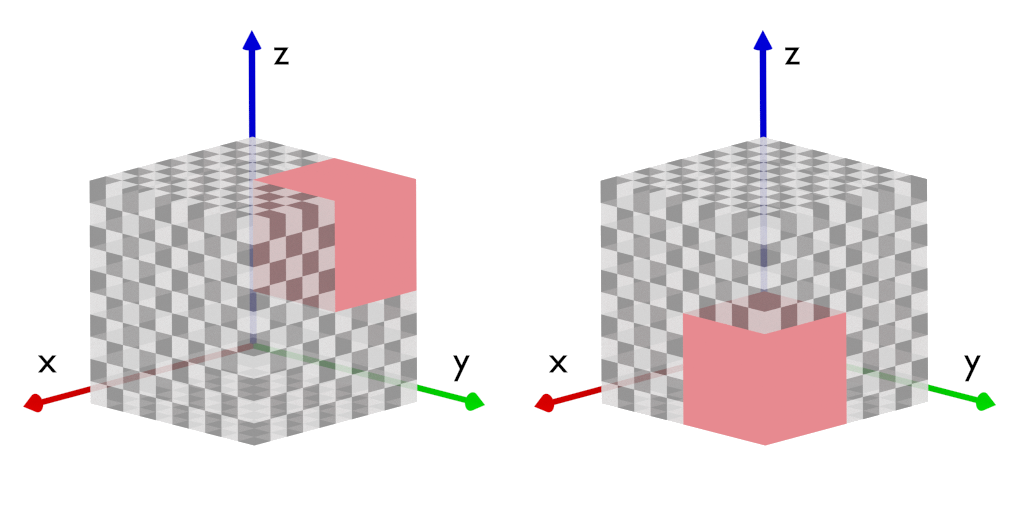
\includegraphics[width=.8\textwidth]{child_node_000_101.png}\\ % PNG-File
  \caption{Parent node (checkered) highlighted child nodes. Left: 000, right: 101}\label{fig:child_node_000_101.png}
\end{figure}

	\texttt{getNodeByIdentifierArray()} returns a reference to an \texttt{ocTree} object whose identifier matches the series of boolean values passed during the call. It mainly served testing and debugging purposes during development of the application, making sure the spatial indexing structure would be computed correctly for any given set of input 3D data. It is a utility function that provides fast, direct acces to any one desired node within an \texttt{ocTree} structure.

	\subsubsection{\texttt{buildTreeRecursively()}}
	\label{sec:buildTreeRecursively}
A call to this function causes an entire set of given vertices to be indexed and assigned leaf nodes in the tree. Its only parameter required is an indexed list of vertices. A \texttt{std::vector<std::pair<size\_t, glm::vec3>>}, with the \texttt{size\_t} parts of the \texttt{pairs} providing ordered indexes and the \texttt{vec3} parts representing the vertices with three coordinates each, is used in this work.

	Most of what this function does, happens in a \texttt{for}-loop which iterates thorugh the entirety of the set of passed vertices. Its basic procedure is depicted in the following simplified C++ code-snippet.

\begin{minipage}{\linewidth}
\begin{lstlisting}[language=C++,numberstyle=\zebra{black!5}{white}{},numbers=left,xleftmargin=2em,tabsize=3]
void ocTree:: buildTreeRecursively(...) {
	for(int t = 0; t != vertices.size(); ++t) {
		it = &vertices[t];
		if (it->second.x >= m_minX && it->second.x < m_maxX) {
			if (it->second.y >= m_minY && it->second.y < m_maxY) {
				if (it->second.z >= m_minZ && it->second.z < m_maxZ) {
					m_verticesInBounds.push_back(*it);
				}
			}
		}
	}

	if (m_verticesInBounds.size() > m_maxVerticesPerNode) {
			if (m_level < m_maxSplitDepth) {
				split();
			} else {
				std::cout << "EXCEPTION" << std::endl;
				return false;
		}
	}
}
\end{lstlisting}
\end{minipage}

Lines 2 - 11 check whether the current vertex lies within the bounds of the calling node. Note that each node calling this function considers every vertex its parent node hold in their member variable \texttt{m\_verticesInBounds}. In turn, if the calling node is to call \texttt{split()} later on, creating eight new subtree nodes, those nodes consider each of the vertices that, via this loop have been determined to be located within their parent node. This stems from the trivial observation that a subtree can only contain vertices that are also contained by their parent node. So the root node of an \texttt{ocTree} always checks every single vertex of the loaded 3D object. However, the higher the level of its subtree nodes, the fewer vertices have to be checked by those nodes.

Line 13 shows the crucial check wheter the number of vertices within the bounds of the calling node exceeds the maximum allowed number of vertices per node. If this is the case and the maximum allowed level (\texttt{m\_maxSplitDepth}) of subtrees is not reached yet (line 13), a call of \texttt{split()} by this node follows.

Figure \ref{fig:ocTree_levels.png} depicts a simple \texttt{ocTree} structure that could result from indexing a small set of 3D data. This particular tree has a root node at level zero, represented as a basic cube in the upper left part of the figure. As the number of vertices within the bounds of the root exceeds the maximum numbers of vertices a node may hold in this particular tree, the root calls \texttt{split()} so that eight new subtrees are created and the root switches its boolean flag \texttt{isLeaf} to \texttt{false}, indicating that it is no longer a leaf node but the root of an actual subtree within the entire \texttt{ocTree}. Given that the maximum level of subtrees visible in the figure is 2, we assume that this is also the maximum allowed level for subtrees. This would mean that the identifier \texttt{vectors} of every node within this tree has a length of $3*2$. The level 1 subtrees 000100 and 000111, as shown in the figure, also have more vertices within their bounds than what is the maximum number of vertices per node so they, too, split and creat a total of 16 new child nodes, each at level 2.

\begin{figure}[htb]
  \centering
  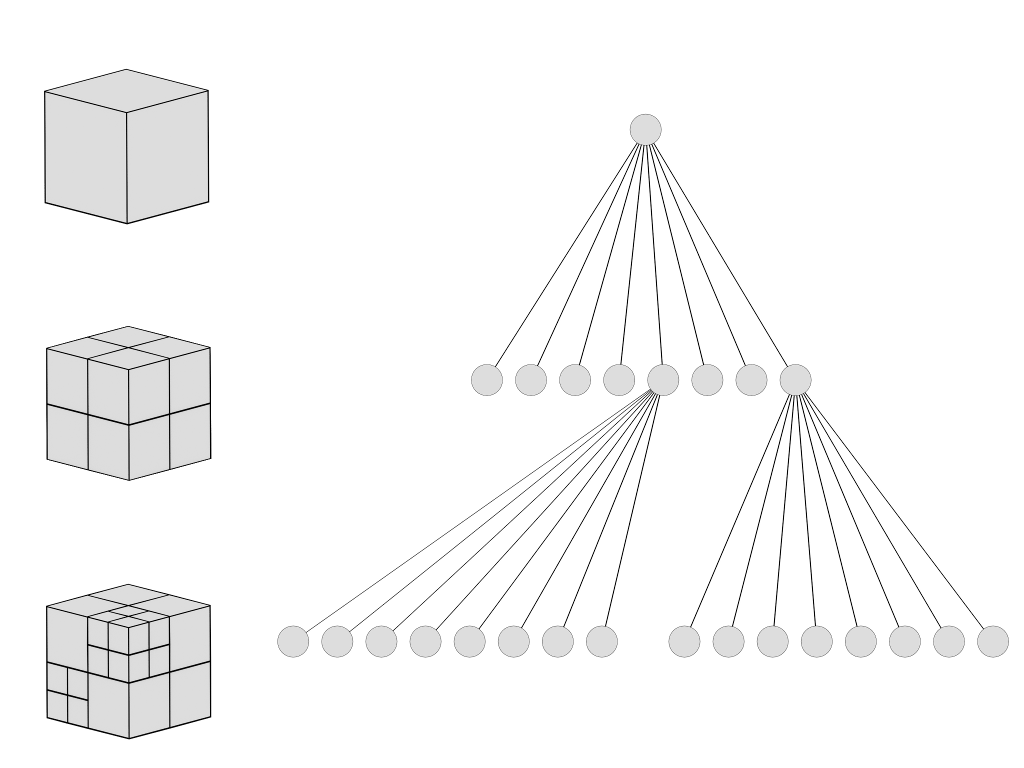
\includegraphics[width=0.95\textwidth]{ocTree_levels.png}
  \caption{depiction of a simple \texttt{ocTree}. Left: 3D view, step-wise representation of the splitting process (downwards from the top). right: final 2D representation of the tree's structure}\label{fig:ocTree_levels.png}
\end{figure}


\pagebreak % @TODO Das im Auge behalten! Zeilenumbruch usw
\subsection{User selection}
\label{sec:user_selection}

This section covers the elementary functions that handle the selection of vertices through user input. The two crucial functions explained in the subsequent subsections implement means to add vertices to an initially empty set of vertices and remove them later if desired. Selected vertices are be visually highlighted in the application and, at any time, the current set of selected vertices can be saved to an external text file.

	\subsubsection{\texttt{addVerticesToSelectionByCoordinates()}}
	\label{sec:addVerticesToSelectionByCoordinates()}
This private, recursive function adds vertices to a set of selected vertices by reference, based on three-dimensional coordinates and a search radius. The following parameters are required:
\begin{enumerate*}
	\item An input coordinate depicting the point in real space where a user is using the input device (a \texttt{glm::vec3} is used in this work),
	\item A \texttt{float} value describing the radius around thee input coordinate in which vertices are to be added to the selection, and
	\item A reference to the set of indexes of vertices (\texttt{std::set<size\_t>} is used in this work)
\end{enumerate*}.

An additional boolean flag determing whether, during the recursive search for the correct node, information is printed to the console or not, is passed with a default value of \texttt{false}. If set to \texttt{true}, it causes information to be displayed. The general course of events within this function proceeds as follows:
\begin{enumerate}
	\item Check if any of the given input point's coordinates are located outside of the bounds of the root of the \texttt{ocTree} indexing the 3D object. Throws exception if this is the case.
	\item Check if the current node is a leaf (i.e. has no child nodes). This terminates the recursive search and proceeds with finding vertices around the given input coordinates, as it is safe to assume that the correct node is found.
	\item Add all vertices within this node to the set of vertices to be checked.
	\item Determine if the radius around the query point crosses the bounds of this node in any direction. If so, add all vertices of the neighbouring node to the set of vertices to be checked.
	\item Iterate over the entire set of vertices to be checked to find which ones lie in radius around the query point and add those to the set of selected vertices.
	\item If this node is not a leaf node - steps 3, 4 and 5 are skipped in this case - determine the correct child node in which the query point is located and have that node recursively call \texttt{addVerticesToSelectionByCoordinates()}.
\end{enumerate}

Consider figure \ref{fig:a01_without_neighbours} for a clear depiction of the process. For the sake of a simplified, clear presentation, an orthographic top view which only considers axes x and y is shown here. Four of an implicitly shown parent node's eight subtree nodes are shown. The figure illustrates, from left to right, three vital steps towards finding vertices that lie within a search radius $r$ around an input query coordinate $P_q$. Throughout these steps, $P_q$ is depicted as an orange point, $r$ is shaded blue. Vertices within this radius compose the result of the query $V_{result}$ and get added to the set of currently selected vertices. Vertices which are considered to get checked if they lay within $r$, $V_{check}$, are highlighted blue, the ones where this is not the case are plain grey.

\begin{figure}[htb]
  \centering
  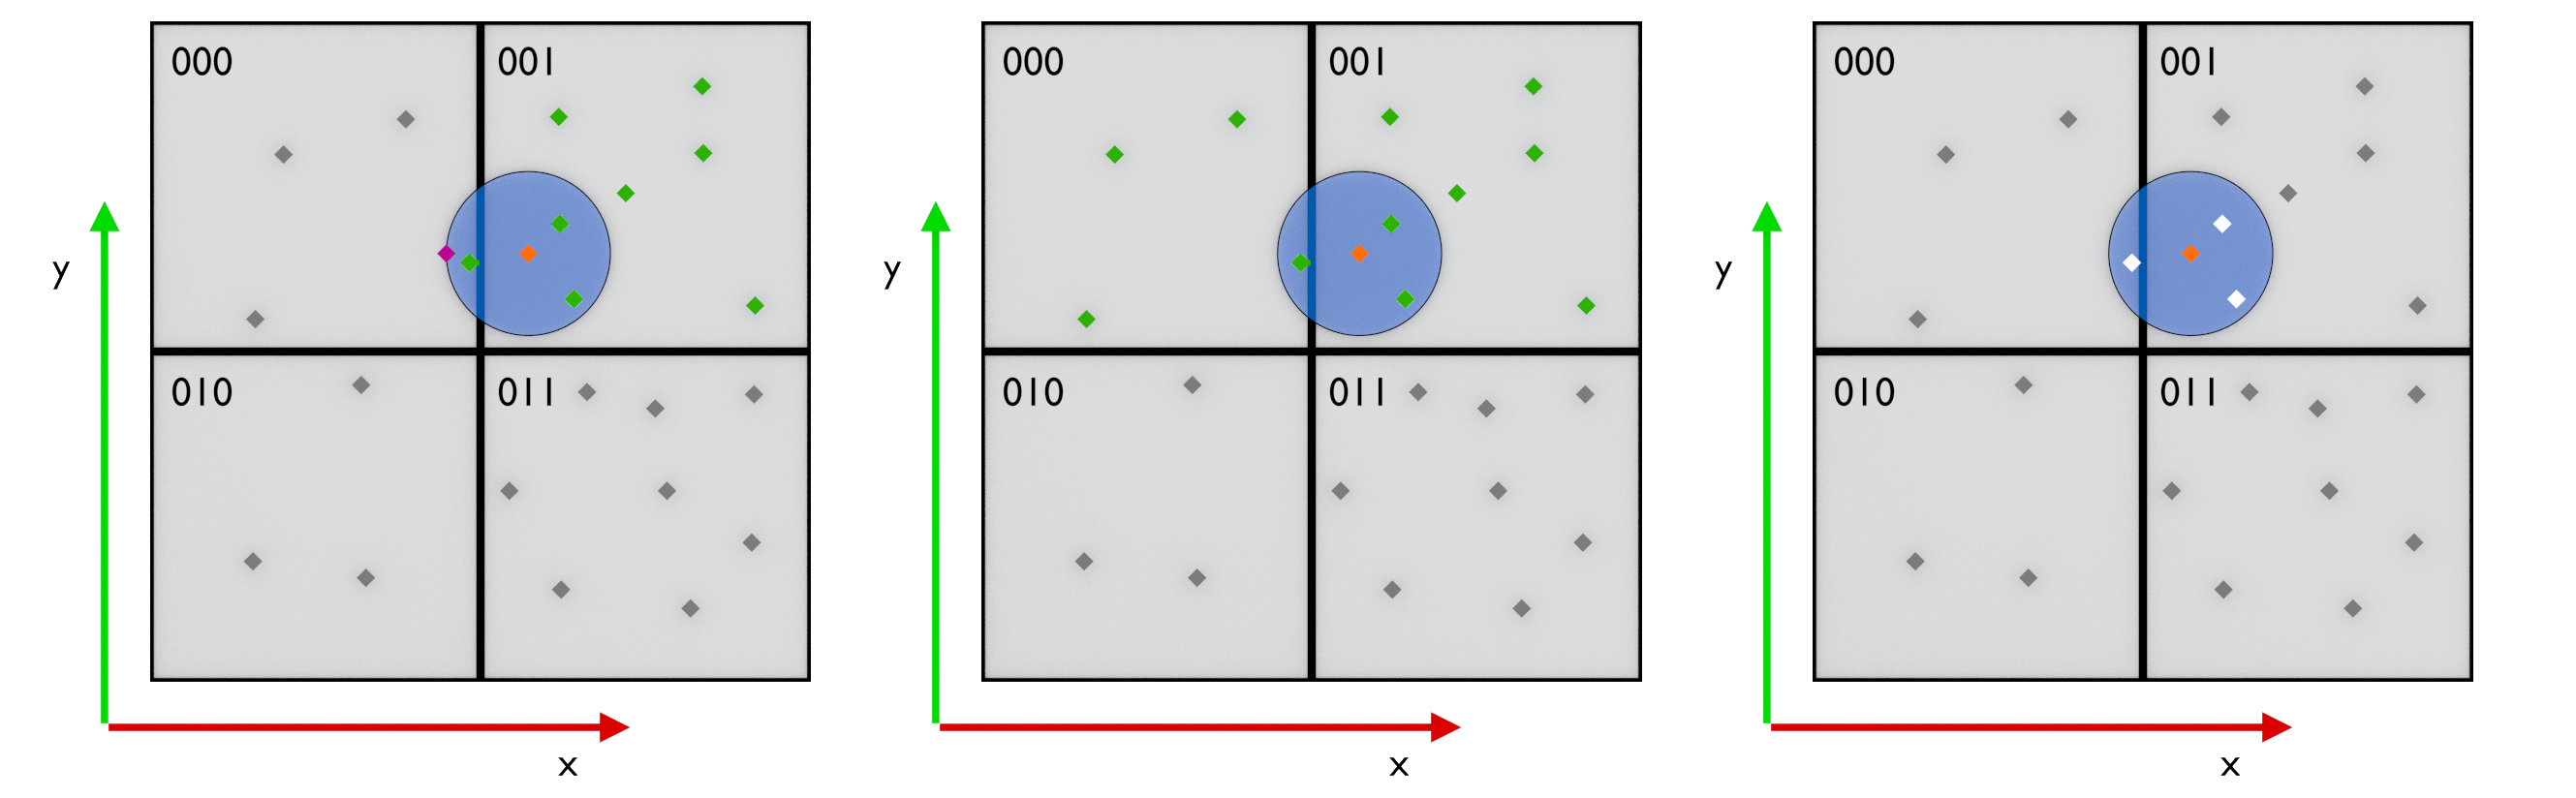
\includegraphics[width=1.0\textwidth]{a01_without_neighbors.png}
  \caption{Determing vertices to check and final set of selected vertices}\label{fig:a01_without_neighbours}
\end{figure}

The leftmost part of figure \ref{fig:a01_without_neighbours} shows the state after two crucial steps have already been taken: Leaf node $N_q$, i.e. the node that contains $P_q$ and does not have child nodes (001 in the figure) is found and all the vertices within it added to $V_{check}$ (highlighted blue). Furthermore, since the search radius around $P_q$ crosses the bounds of $N_q$ in negative x direction, an additional call to \texttt{addVerticesToSelectionByCoordinates()} with parameters $P_{q}^{'}$ and radius $r^{'}$ = 0 is executed, with $P_{q}^{'}$ = [$P_q.x-r$, $P_q.y$, $P_q.z$] (highlighted purple). This additional query found that $P_{q}^{'}$ is located in leaf node 000. Thus, as shown in the middle part of the figure, vertices in 000 are added to $V_{check}$. Note that one vertex that is located within $r$ - but not the bounds of $N_q$ is added to $V_{check}$ this way. The righthand part of the figure shows the result of the original query. After checking all vertices in $V_{check}$ whether they lie within $r$ around $P_q$, a set of vertices which fulfill this very condition $V_{result}$, containing three vertices (highlighted white) is returned.

The following code-snippets show how the process described above is implemented in this work.

\begin{minipage}{\linewidth}
\begin{lstlisting}[language=C++,numberstyle=\zebra{black!5}{white}{},numbers=left,xleftmargin=2em,tabsize=3]
ocTree* ocTree::addVerticesToSelectionByCoordinates(...) {
	if (target.x < m_minX || target.x > m_maxX || target.y < m_minY
		|| target.y > m_maxY || target.z < m_minZ || target.z > m_maxZ) {
		std::cout << "EXCEPTION" << std::endl;
		return NULL;
	}

	if (this->getisLeaf() == true) {
		result = this;
		std::vector<std::pair<size_t, glm::vec3> > verticesToCheck;
		for(size_t t = 0; t < result->m_verticesInBounds.size();++t){
			verticesToCheck.push_back(result->m_verticesInBounds[t]);
		}
		if (radius != 0) {
			glm::vec3 neighbourCo;
			if (target.x - radius < m_minX) {
				neighbourCo = {target.x-radius, target.y, target.z};
				ocTree * neighbour = m_root->addVerticesToSelectionByCoordinates
				(neighbourCo,0,intermediateSelection,debugInfo);
				verticesToCheck.insert
				(verticesToCheck.end(), neighbour->m_verticesInBounds.begin(),
				neighbour->m_verticesInBounds.end());
			}
			if (target.x + radius > m_maxX) {
				neighbourCo = {target.x+radius,target.y,target.z};
				ocTree * neighbour = m_root->addVerticesToSelectionByCoordinates
				(neighbourCo,0,intermediateSelection,debugInfo);
				verticesToCheck.insert
				(verticesToCheck.end(), neighbour->m_verticesInBounds.begin(),
				neighbour->m_verticesInBounds.end() );
			}
			// <repeat for y and z direction>
		}

		std::vector<std::pair<size_t, glm::vec3>>::const_iterator it;
		for (it = verticesToCheck.begin(); it!=verticesToCheck.end(); ++it) {
			if (radiusContainsCoordinates(r, it->second) {
				intermediateSelection.insert(it->first);
			}
		}
		return result;
	}
}
\end{lstlisting}
\end{minipage}

In lines 2 - 6, it is validated whether the input coordinates of $P_q$ given via \texttt{target} is located within the bounds of the calling node - that is usually going to be the root node of an \texttt{ocTree} structure. If this is not the case, \texttt{null} is returned.
If line 8 evaluates to \texttt{true}, this means that the current node is a leaf node and since given input coordinates do not lie outside its bounds, this has to be target node of the query $N_q$.

In line 10 - 13, a new \texttt{vector} of \texttt{pairs} consisting of \texttt{size\_t} values and \texttt{glm::vec3} vectors, representing the set of vertices to be checked is created. The \texttt{size\_t} parts of  \texttt{pairs} in this vector provide unique indexing, ensuring fast and direct access to each element. However, at this stage, this set only contains vertices within initial target node $N_q$. Without the rest of the code, vertices within one or multiple \textit{neighbour nodes} that contain $P_{q}^{'}$ vertices which sould get selected, would be ignored.

Line 14 - 36 show two out of six possible types of \textit{neighbour node queries} - both possible ways in which \textit{r} can cross the bounds of $N_q$ in x direction and how they are handled are illustrated. Note how parameter \texttt{radius} is used here (line 14). If it is set to 0, this request (which is also handled by \texttt{addVerticesToSelectionByCoordinates} can be classified as a \textit{neighbour query} which means that it cannot possibly envoke further \textit{neighbour queries}. In lines 17 and 28, varying intermediate versions of $P_{q}^{'}$ are derived by adding and subtracting \texttt{radius} to initial x value of $P_{q}$ after it is found that they are located within a neighbouring node of $N_q$ (lines 16 and 24). After this, assitional queries are processed via \texttt{addVerticesToSelectionByCoordinates} with crucial input parameters $P_{q}^{'}$ and \texttt{radius} = 0 (lines 18, 19 and 26, 27). Finally, the vertices within the found \textit{neighbour node} are added to the set of vertices to be checked (lines 20 - 22 and 28 - 30). As hinted by the comment in line 32, this process is repeated for y and z directions.

Before recursively returning the calling node in line 41, the most important part of this function - that is actually determining which vertices are located in raidus \textit{r} around input coordinates $N_q$ - takes place in lines 36 - 40. Here, we see a \texttt{for} loop through $V_{check}$, the set of vertices that lie within the bounds of $N_q$ as well as those within one or more \textit{neighbour nodes} $N_q^{'}$. The simple utility function \texttt{radiusContainsCoordinates} takes care of this. Note that, in case it evaluates to \texttt{true}, the \texttt{first} element of a pair within \texttt{verticesToCheck} (or $V_{check}$) is added to \texttt{intermediateSelection} (or $V_{result}$). This first element is a simple \texttt{size\_t} number which serves as a unique identifier for every vertex of the entire loaded object. This approach ensures that almost negligibly small amounts of data are actually transferred within the application - between server to client instances (see
\ref{sec:selection_process})
). Depending on what system architecture the application is ran on, these \texttt{size\_t} values only take 32 or 64 bits of space in memory, whereas \texttt{glm::vec3} take up to 12 times as much space.

Note that the code-snippet above only considers cases in which \texttt{radius} $r$ around $N_q$ crosses one set of bounds of \texttt{ocTree} nodes. However, it is a trivial observation of the conceptual structure of octrees that, depending on combinations of a large \texttt{radius}, a low maximum allowed number of vertices per node and a high maximum allowed \texttt{level}, critical situations could emerge. Such a situation could take place in a fine-grained octree structure with a large number of high level leaf nodes. For any node $N$ on a level $l$, the following is true.

$N_s$($d$) = $N_{R}$($d$) / $2^{l}$ where $N_s$($d$) is the size of $N$ in dimension $d$ and $N_{R}$($d$) is the size of root node $N_{R}$ in dimension $d$.

So in this application, after the object is loaded and spatially indexed, we consider the maximum allowed level for leaf nodes $l_{max}$ as well as the bounding values of its root node. The minimum difference between the maximum and mininum values in a dimension indicate the shortest dimension $d_{min}$ of the root node. Based on these values, we can set a maximum allowed value $r_{max}$ for the search radius as follows.

$r_{max}$ = $d_{min}$ / $2^{l_{max}}$ * 0.95. In other words, the maximum allowed search radius is 95\% the size of the smallest possible leaf node. Thus, no search query can evoke more than three additional queries for \textit{neighbour nodes}, one in each dimension.

Finally, the following simplified code-snippet shows how, making use of recursion, child nodes perform further calls to \texttt{addVerticesToSelectionByCoordinates} until $N_q$ (or $N_{q}^{'}$) is found, based on the directions in which $P_{q}^{'}$ crosses the bounds of the calling node.

\begin{minipage}{\linewidth}
\begin{lstlisting}[language=C++,numberstyle=\zebra{black!5}{white}{},numbers=left,xleftmargin=2em,tabsize=3]
ocTree* ocTree::addVerticesToSelectionByCoordinates(...) {
	// <cont.>
	if (target.x < m_meanX) {
		if (target.y < m_meanY) {
			if (target.z < m_meanZ) {
				// 110
				result = m_myChildren[6]->addVerticesToSelectionByCoordinates();
			} else {
				// 010
				result = m_myChildren[6]->addVerticesToSelectionByCoordinates();
			}
		} else {
			if (target.z < m_meanZ) {
				// 100
				result = m_myChildren[6]->addVerticesToSelectionByCoordinates();
			} else {
				// 000
				result = m_myChildren[6]->addVerticesToSelectionByCoordinates();
			}
		}
	} else {
		if (target.y < m_meanY) {
			if (target.z < m_meanZ) {
				// 111
				result = m_myChildren[6]->addVerticesToSelectionByCoordinates();
			} else {
				// 011
				result = m_myChildren[6]->addVerticesToSelectionByCoordinates();
			}
		} else {
			if (target.z < m_meanZ) {
				// 101
				result = m_myChildren[6]->addVerticesToSelectionByCoordinates();
			} else {
				// 001
				result = m_myChildren[6]->addVerticesToSelectionByCoordinates();
			}
		}
	}
}
\end{lstlisting}
\end{minipage}

Finding which child node $N_{l+1}$ is to perform the next recursive call happens in three simple \texttt{if - else} statements, the first one consisting of blocks of lines 3 - 20 and 21 - 39. In case the first \texttt{if} in line 3 evaluates to \texttt{true}, $P_q$ lies between the calling subtree node's minimum and mean values in x direction, thus the relevant child node's identifier must be \texttt{false} (0) at its \textit{level offset} $O_{l+1}$+2. If the statement in line 4 is \texttt{true}, the second $O_{l+1}$+1 can only be \texttt{true} (1). Whether the last value at $O_{l+1}$ is \texttt{true} or \texttt{false} is determined in line 5. We see exemplary, shortened recursive calls to \texttt{addVerticesToSelectionByCoordinates} in lines 7, 10, 13, 15, 18 and so on which are returned at the end of the function.

	\subsubsection{\texttt{removeVerticesFromSelectionByCoordinates()}}
	\label{sec:removeVerticesFromSelectionByCoordinates()}

This is the counterpart to \texttt{addVerticesToSelectionByCoordinates} and the second of two elementary methods that allow users to create and modifiy vertex selections in this application. Using the exact same parameters in identical order, it is a private, recursive function that allows for vertices added to the current selection to be removed again. In fact, the two functions vary so little, we can use the same list of general tasks as shown in \ref{sec:removeVerticesFromSelectionByCoordinates()}. The crucial differences are highlighted in bold text.

\begin{enumerate}
	\item check if any of the given input point's coordinates are located outside of the bounds of the root of the \texttt{ocTree} indexing the 3D object. Throws exception if this is the case.
	\item check if the current node is a leaf (i.e. has no child nodes). This terminates the recursive search and proceeds with finding vertices around the given input coordinates, as it is save to assume that the correct node is found.
	\item add all vertices within this node to the set of vertices to be checked.
	\item determine if the radius around the query point crosses the bounds of this node in any direction. If so, add all the vertices of the neighbouring node to the set of vertices to be checked.
	\item iterate over the entire set of vertices to be checked to find which ones lie in radius around the query point and \textbf{remove those from} the set of selected vertices.
	\item if this node is not a leaf node - steps 3, 4 and 5 were skipped in this case - determine the correct child node in which the query point is located and have that node recursively call \textbf{\texttt{removeVerticesFromSelectionByCoordinates()}}.
\end{enumerate}

At this point it is worth noting that these two fundamental functions were mapped to two different buttons on the handheld controller used at the V2C. Figure \ref{fig:selection.png} shows a simple 3D object at various stages during consecutively performing these fundamental operations on it. The leftmost part of the figure shows a simple sphere with no vertices selected. The middle part shows the same sphere after eight vertices have been added to the selection and how they are highlighted. The righthand part of the figure shows the object after four vertices have been removed from the selection via \texttt{addVerticesToSelectionByCoordinates} with other coordinates.

\begin{figure}[htb]
  \centering
  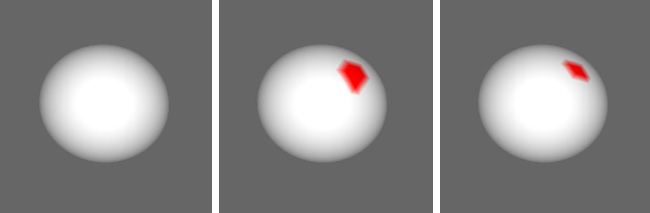
\includegraphics[width=0.9\textwidth]{selection.png}
  \caption{A basic vertex selection process}\label{fig:selection.png}
\end{figure}


\subsection{Tracking selection}
\label{sec:tracking_selection}

The set of user selected vertices is being kept track of as described in this section. Using the two fundamental functions described in \ref{sec:removeVerticesFromSelectionByCoordinates()} and \ref{sec:addVerticesToSelectionByCoordinates()}, every vertex of a spatially indexed 3D object can be selected and deselected at will. At each frame, every currently selected vertex is highlighted in an easily distinguishable bright red shade. Additionally, at any point during runtime, the server program of the application can print the current set of selected vertices to an external textfile.

Vertices in this application can either be selected or not selected. Only selected vertices are tracked. This is implemented using the following two variables in the main class.

\begin{description}
	\item[\texttt{std::set<size\_t> vertexSelection}] - a set of unsigned integers. A \texttt{set} is a C++ specific type of container with two handy properties for this use case. It guarantees the uniqueness of each element, as the value of an element is also the key used to identify it, and it is allocator-aware, which means it uses an allocator object to dynamically handle its storage needs (see \cite{set}).
	\item[\texttt{std::vector <std::pair <size\_t, glm::vec3> >  verticesList}] - A \texttt{vector} containing \texttt{pairs} of unique \texttt{size\_t} values and \texttt{glm::vec3} objects. \texttt{vectors} are contiguous storage containers that can store any type of objects, provide access to elements by using offsets (just like arrays) but also change their size dynamically (see \cite{vector}). Since the actual content of this variable is created and stored during spatially indexing a loaded 3D object during the recursive building process of an octree structure (see \ref{sec:buildTreeRecursively}), its final required size is not know at startup of the application, hence an ordinary \texttt{array} is not a suitable datatype here.
\end{description}

After the setup process of the application, \texttt{verticesList} essentially holds an ordered list of pairs of integer numbers and three-dimensional coordinates. Table \ref{tab:verticesList-startup} illustrates an excerpt of its possible content after startup. Note that the order of coordinates is arbitrary and, in no way, represents the structure or order of the loaded 3D file.

\begin{table}[]
\centering
	\begin{tabular}{l|l}
	offset (\texttt{size\_t}) & coordinate (\texttt{glm::vec3}) \\ \hline
	0 & [0.481, 0.461, 0.458] \\
	1 & [0.351, 0.335, 0.024] \\
	2 & [0.385, 0.324, 0.021] \\
	3 & [0.452, 0.342, 0.125]
	\end{tabular}
	\caption{content of \texttt{verticesList} at startup}
	\label{tab:verticesList-startup}
\end{table}
% table 4.3

% print, genaueres zu add und remove in der CAVE, globales set von size_t und vec3s

\subsection{Testing setup}
\label{sec:testing_setup}
% Helper- & Debug-Funktionen; Blend-File; Eigenhändige Tests in CAVE(?)

This section describes the steps taken to ensure that the selection application meets all its requirements and ensures its key features described above are implemented correclty. While it is not formally verified that the application works correctly in every use case conceivable, it was tested up until a point where fluent, real-time and comfortable interaction was possible from a user perspective.

		\subsubsection{Test files}
		\label{sec:test_files}
While developing the selection application, I used 3D modeling software to create a set of simple test files that would be exported to .obj format so they could be used for testing purposes. These objects were designed to test whether common queries are handled quickly and correctly as well as what happens in unfortunate edge cases. Such a fairly complex edge case is depicted in figure \ref{fig:edge_case}.

\begin{figure}[htb]
  \centering
  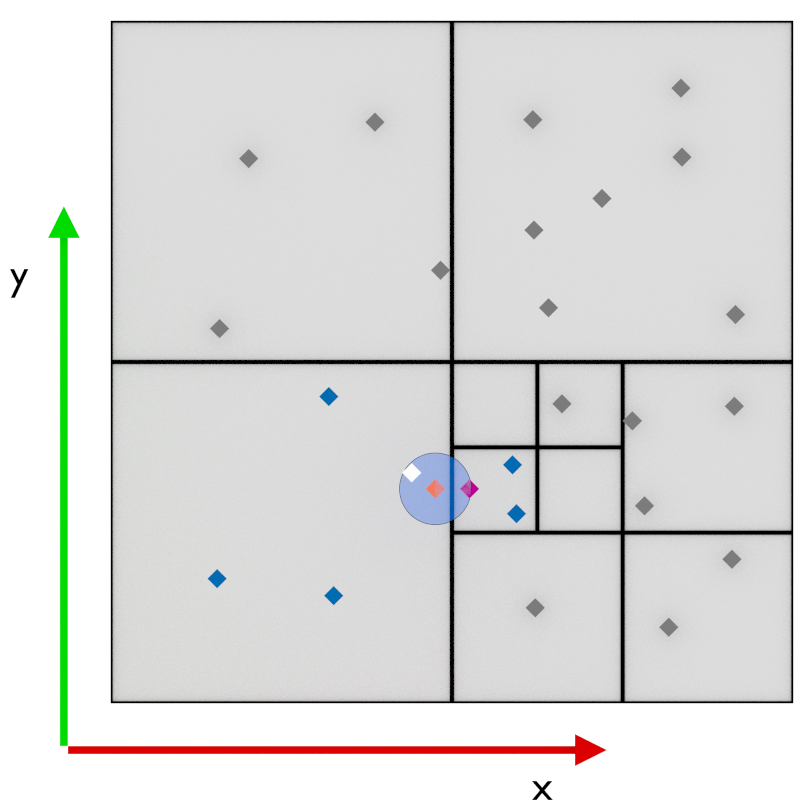
\includegraphics[width=0.5\textwidth]{edge_case.png}
  \caption{A fairly complex query to the octree structure of the selection application}\label{fig:edge_case}
\end{figure}

For the sake of readabilty, figure \ref{fig:edge_case} depicts an orthographic view on the structure of a test file used, showing only x and y axes. In such a case, all vertices shaded blue must be considered but only the one vertex shaded white is a correct result to the query. An additional query with input coordinates depicted by the point shaded in purple and radius 0 must be invoked and correctly handled as well, since the righthand border of the target subtree is crossed by the search radius. All vertices shaded grey must not be considered. The behavior of the application must be congruent to what is described in section \ref{sec:additional_third_party_libraries}.

\begin{figure}[htb]
  \centering
  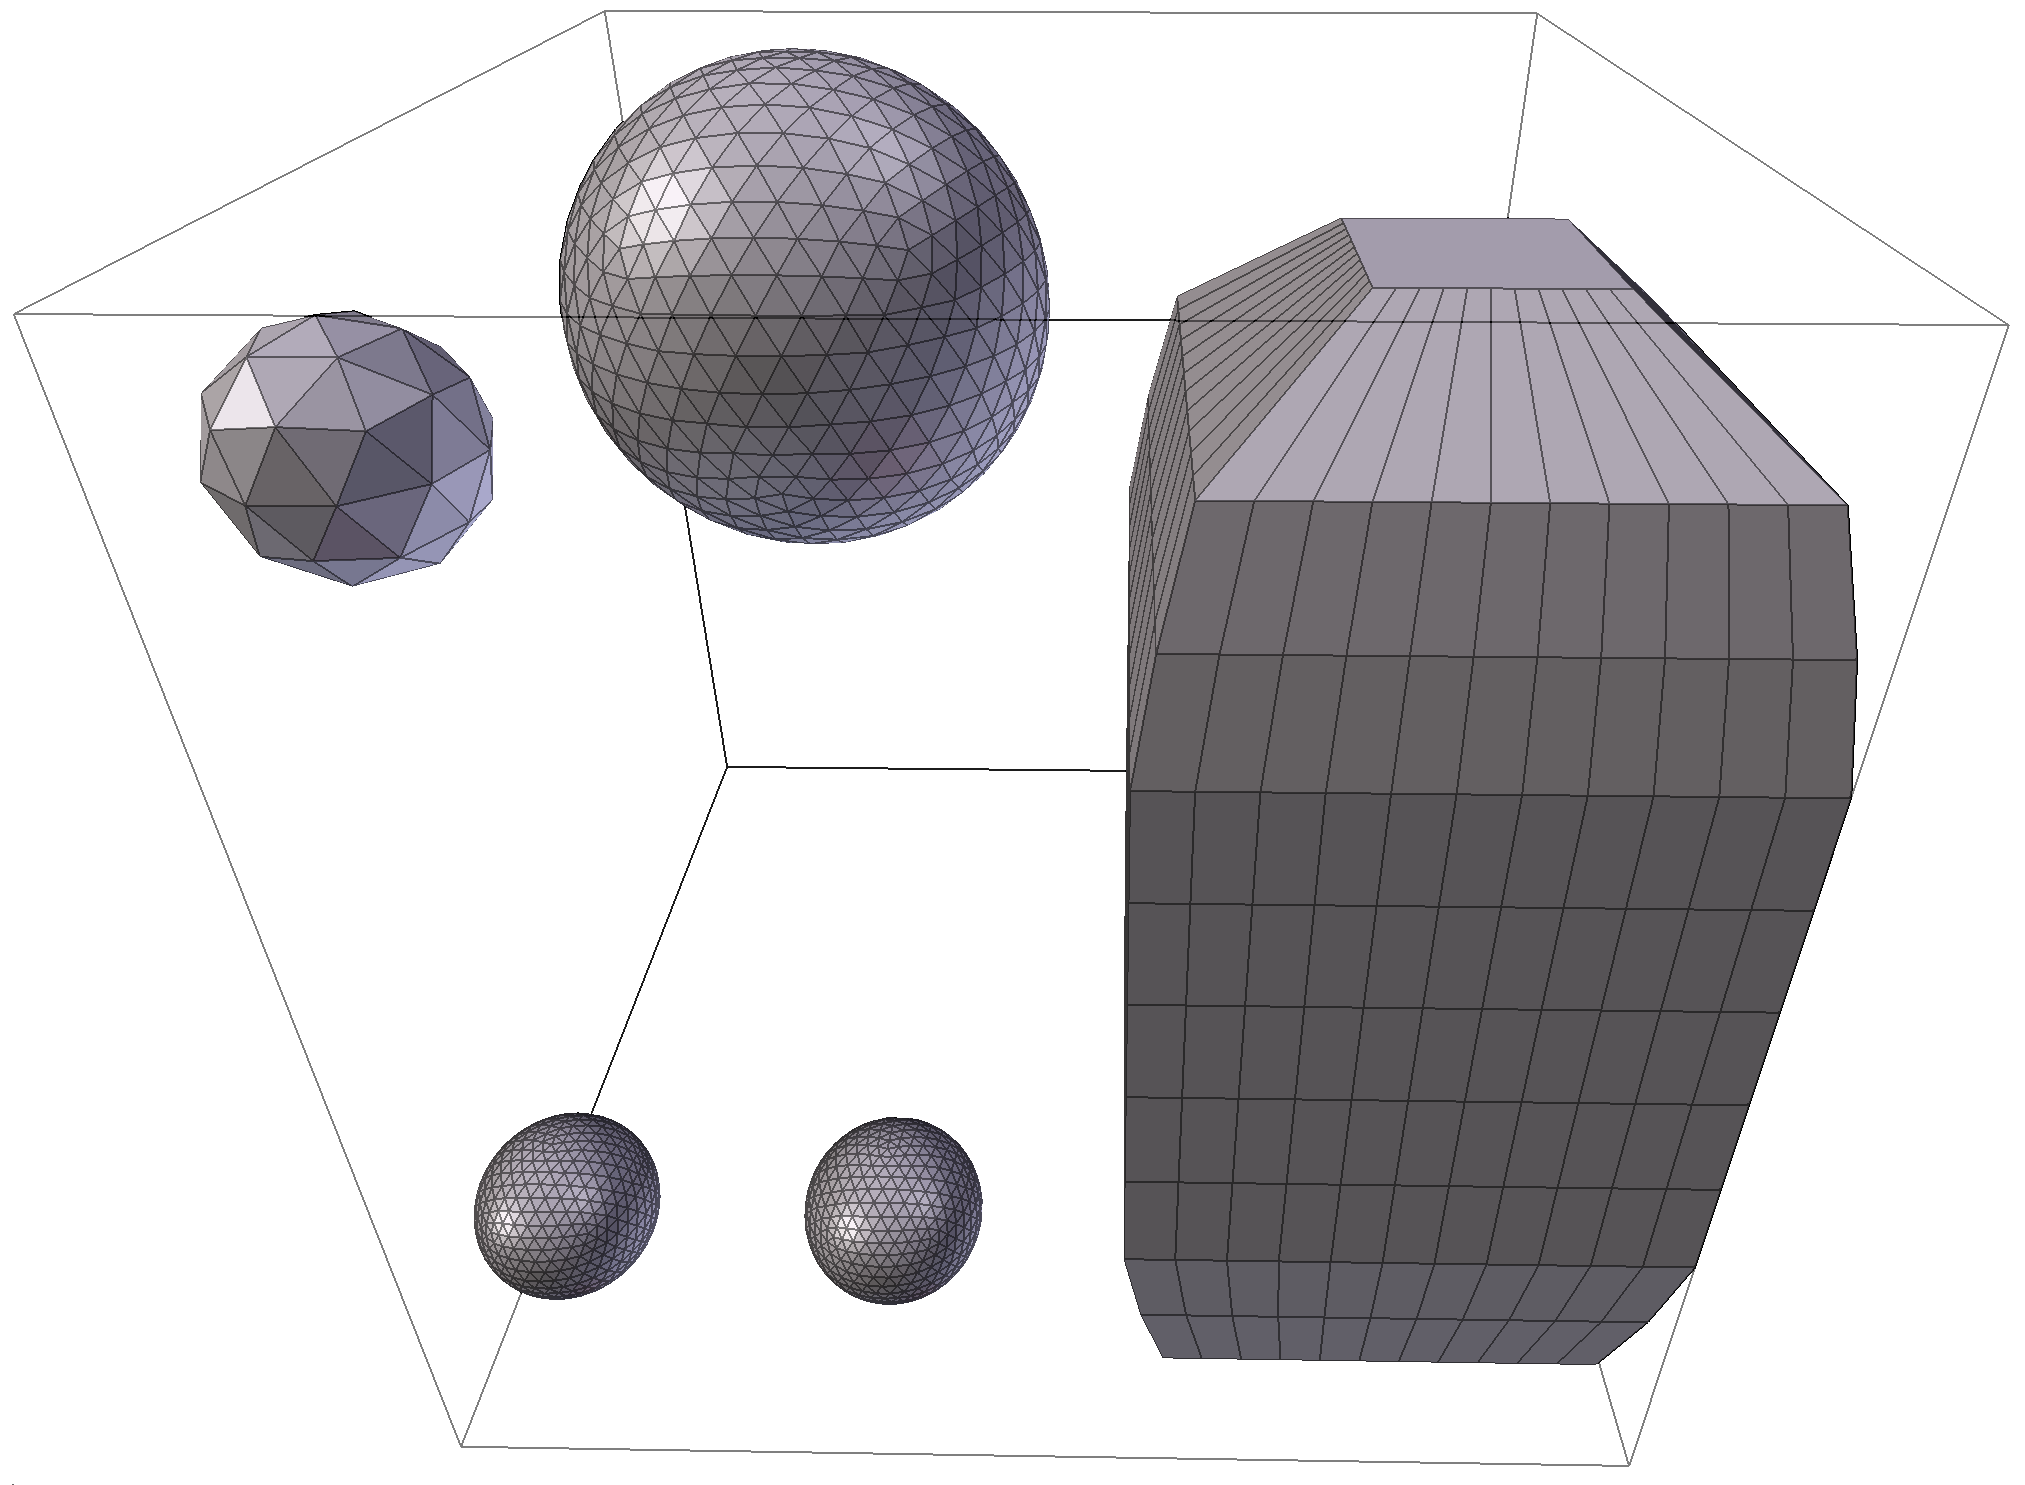
\includegraphics[width=0.75\textwidth]{test_file.png}
  \caption{A test file used during implementation, perspective view. Its bounding box and edges are depicted}\label{fig:test_thing}
\end{figure}

Figure \ref{fig:test_thing} shows a test file used during all stages of implementing the selection application. It is designed for the Octree structure to be built in a clearly predictable way. For each combination of the maximum allowed number of vertices per node and the maximum allowed level, construction of the structure can be precicely predicted because all parts of the object are positioned in eighths of the space encapsulated by its bounding box. This file was used to a great extent for many testing queries as well as debugging.

The debugging process encompassed a multitude of test calls to the applications core functions using arbitrary coordinates as well as extensive use of the helper and debugging functions described in the subsequent subsection.

		\subsubsection{Helper and debugging functions}
		\label{sec:helper_and_debugging_functions}
The following functions which are non-essential to the functionality of the application are included. They were used during implementation for documentation, debugging and controlling the correctness of the core features. Parameters for these functions are omitted.

\begin{description}
	\item[\texttt{ocTree* getNodeByIdentifierArray()}] - gets a leaf node via a boolean input array representing its identifier. Traverses through an entire tree and returns the node with given identifier at the lowest level. The input boolean array has to contain $3*$ the maximum allowed split depth boolean values representing the identifier of a node. For example, at a maximum allowed split depth of 3, \texttt{false, false, false, true, true, false, false, true, true} is interpreted as 000110011 and a pointer to the according leaf node is returned.
	\item[\texttt{bool getIsLeaf()}] - determines whether this is a leaf or not. Returns private bool variable \texttt{m\_isLeaf}.
	\item[\texttt{void debugTreeInfo()}] - prints information about the finished \texttt{ocTree} object to the console, including total number of vertices stored by it, maximum allowed number of vertices per leaf, maximum allowed split depth and dimensions in x, y and z direction.
	\item[\texttt{void debugFirstVertex()}] - prints the coordinates of vertex at index 0 \texttt{m\_vertices} to the console. This is a quick way to verify that import via ASSIMP worked.
	\item[\texttt{debugAllVertices()}] - prints the coordinates of all vertices to the console. This is a way to verify that import via ASSIMP worked correctly.
	\item[\texttt{void debugIdentifierasString()}] - prints the boolean identify array of the calling subtree to the console in an easily readable form, i.e. 001101 for example. If the calling node is the root, "I am root" is printed instead. Additionally, \texttt{m\_level} as well as the identifer array of the parent node of the calling subtree node are printed.
\end{description}

In addition, all essential functions of the \texttt{ocTree} class have an optional parameter \texttt{debugInfo}, which is set to \texttt{false} by default. If set to \texttt{true}, information is printed to the console during execution of the functions. Depending on what function is called, this information varies strongly obviously. In general, all subtree nodes that recursively call any relevant functions as a result of the initially called function, call \texttt{debugIdentifierasString()}.

		\subsubsection{Testing at the V2C}
		\label{sec:testing_at_the_v2c}

I spent multiple hours in the projection installation, trying the application myself. By experiencing the application from a user perspective, I wanted to make sure the feedback is quick, clearly noticable and easiyl understandable. I tried to find bugs and wrong behavior by using the hardware in ways that were not planned on. Formally describing the procedure does not make sense, so consider the following brief descriptions of things I tried and what insights I gathered from them.

\begin{description}
	\item[Finding limitations to the tracking setup] - The projection installation of the V2C is 2.7 meters in width, height and depth. I tried to find out where the tracking system was working reliably and precisely and where the tracked space ended. I did not take exact measures but I found out that at a distance of about 30 centimeters away from the walls and the floor, the tracking started to get inaccurate. The positions of the tracked devices would freeze at the last position it was tracked correctly, thus making further selection or deselection operations impossible as well as leading to wrong projection of the scene.
	\item[Finding limitations to response time] - At a slow pace of movements, the projection thrown onto the walls surrounding the user, the visual feedback on where selection operations take place as well as indication of their results are in perfect synchronisation with what a user would expect. However, when moving the handheld input device rapidly, its tracked position would get corrupted and the bright green object indicating its position within the 3D scene would only be rendered every dozen or so frames, being frozen in place in the meantime.
	\item[Finding limitations to synchronisation] - During the selection process and during the user study, the application froze multiple times. One or more projection programs would not react anymore, leaving no option but force-quitting and restarting the application. I was not able to reproduce this behavior. I can only speculate, based on various times trying this myself, that if a button is pressed for an ongoing timespan while rapidly moving the handheld input device, this behavior seemed to occur mor frequently. Again, a formal description of what happened as well as the reasons why it happened can not be provided. A more extended testing and bugfixing process would be needed and this goes beyond the scope of this work.
	\item[Evaluating immersiveness and projection quality] - As described in section \ref{sec:technical_issues}, the framerate of the projection onto the the top wall was noticeably higher than those of the other projectors. During the user study, no remarks regarding this were made but from a developer stance, this can potentially impair immersion. Upon taking a look as close as possible to details of projected objects, the overlay of the two projections became visible, causing an incorrect spatial effect and blurriness. However, this only was noticeable when the tracked stereoscopic glasses got really close to the surface of a projected model.
\end{description}

In conclusion, it is fair to say that the \textit{selection application} provides clear feedback on what is happening based on user interaction and interaction is possible at a not too fast movement speed. Users should keep in mind that the tracking system has limitations. Not getting close to walls and not moving the handheld input device rapidly while simultaneously keeping buttons pressed ensures a convenient, fluent interaction.

